\documentclass[11pt, a4paperm, hidelinks]{article}
\usepackage[utf8]{inputenc}
\usepackage[T1]{fontenc}
\usepackage[english]{babel}
\usepackage{lmodern}


\usepackage[a4paper,top=3cm,bottom=3cm,left=3cm,right=3cm]{geometry}
\usepackage{chngcntr}

%package used to enumerate figures
\usepackage[labelfont=bf]{caption}

%hyperref for interactive PDF index
\usepackage[bookmarks, colorlinks, breaklinks]{hyperref}
\hypersetup{linkcolor=black, citecolor=black, filecolor=black, urlcolor=black}

%Package required to use special symbols
\usepackage{amsmath, amssymb}

%Package required to use figures
\usepackage{graphicx}
\usepackage{subfig}
\usepackage{placeins}
\usepackage{wrapfig}

%Include the bibliography in the table of contents
\usepackage{tocbibind}

%Package used to insert figures at the specified position
\usepackage{float}
\usepackage{longtable}

\usepackage{times}

%Our chapters must be called sections
\addto\captionsenglish{\renewcommand{\chaptername}{Section}}

%Header
\usepackage{fancyhdr}
\pagestyle{fancy}
\fancyhf{}
\rhead{Stefano Bagarin - Alessandra Pasini}
\lhead{Design Document}
\rfoot{Page \thepage}

\begin{document}

	%Code for title page
	\begin{titlepage}
		\centering
		
\includegraphics[width=0.20\textwidth]{./assets/polimi-logo.png}\par

		{Politecnico di Milano \\ AA 2019/2020} \par
		\vspace{1.5cm}

		{Computer Science and Engineering}\par
		\Large{Hypermidia Applications}\par
		\vspace{1.0cm}

		{\LARGE \textbf{Design Document} \par}
		\vspace{1.5cm}

		{\normalsize {\textbf{Stefano Bagarin}: mrt. 945159 -  stefano.bagarin@mail.polimi.it }\par}
		\vspace{0.2cm}
		{\normalsize{\textbf{Alessandra Pasini}: mtr. 920051 - alessandra.pasini@mail.polimi.it}\par}
		\vspace{1.0cm}
		
		{\normalsize {\textbf{Inspected website}: \url{Our website if we started already}}\par}
		\vspace{0.2cm}
		{\normalsize {\textbf{Delivery Date}: tbd}\par}
		\vfill

		% Bottom of the page
		{\large Document version: 1.0\par}
		{\large \today \par}
	\end{titlepage}

	%Make the table of contents
	\tableofcontents
	\clearpage


	%Abstract
	\section{Abstract}
	The aim of this document is to report the Inspection-based Usability Evaluation of \emph{Visit Monterosa} website which can be found at the following url \url{https://www.visitmonterosa.com/}. \\ TODO: The analysed website provides extensive
information about the Natural Park of Adamello – Brenta including descriptions of local history
and environment, activities and attractions available in the park paired with an interactive map of
tracks, initiatives organized by the park authorities and much more. The contents include an
analysis on through heuristic inspection of XX expert evaluators and an overall evaluation of the
product along with our conclusions. The Annex provides the individual scores of each inspector.


goal 1 : trovare esperienze e pronarle   “Searching information about experiences and opportunities”
goal 2 : prenotare vacanza 
goal 3 : avere informazioni sul monterosa
	\clearpage


	%Graphical Representation
	\section{Graphical Representation}

	\subsection{C-IDM}
	\begin{figure}[h!]
		\centering
		\begin{minipage}[b]{1\textwidth}
    			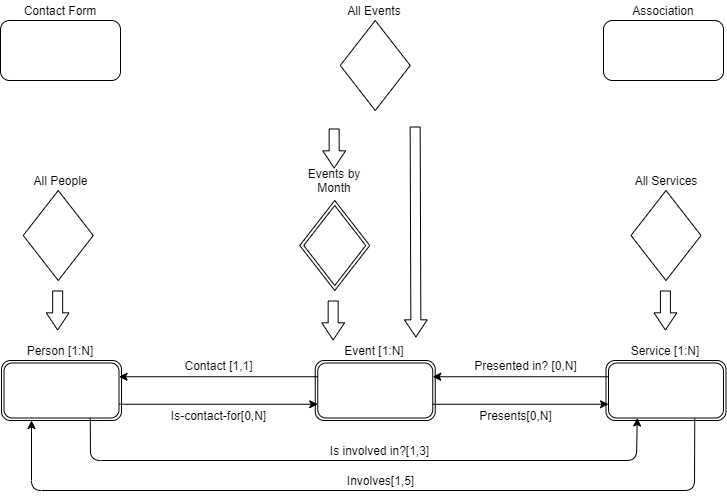
\includegraphics[width=\textwidth]{./assets/C-IDM.png}
			\caption{Content Interactive Dialogue Model}
		\end{minipage}
	\end{figure}
	\FloatBarrier
	\clearpage

	\subsection{L-IDM}
	\begin{figure}[h!]
		\centering
		\begin{minipage}[b]{1\textwidth}
    			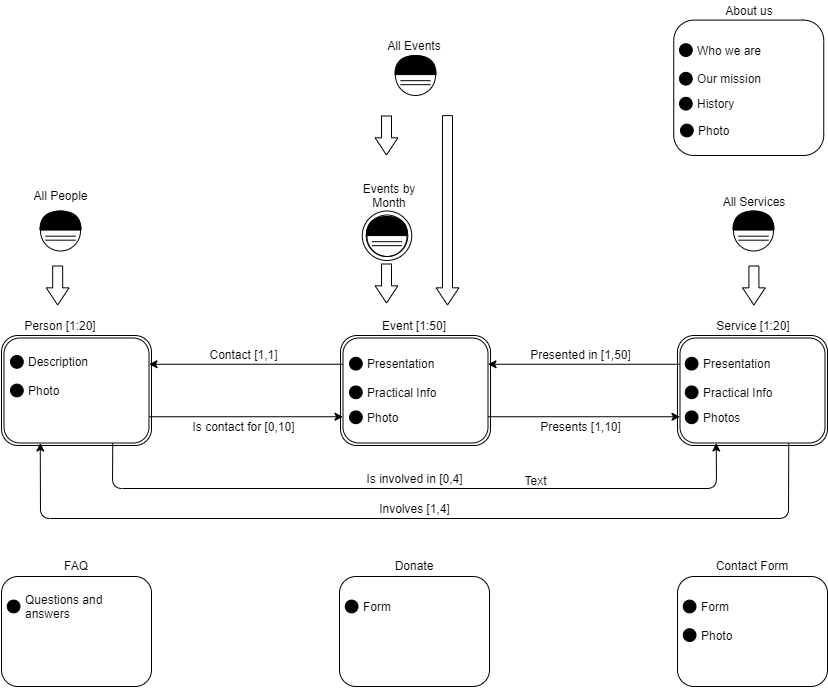
\includegraphics[width=\textwidth]{./assets/L-IDM.png}
			\caption{Logical Interactive Dialogue Model}
		\end{minipage}
	\end{figure}

	\subsection{P-IDM}
	\begin{figure}[h!]
		\centering
		\begin{minipage}[b]{1\textwidth}
    			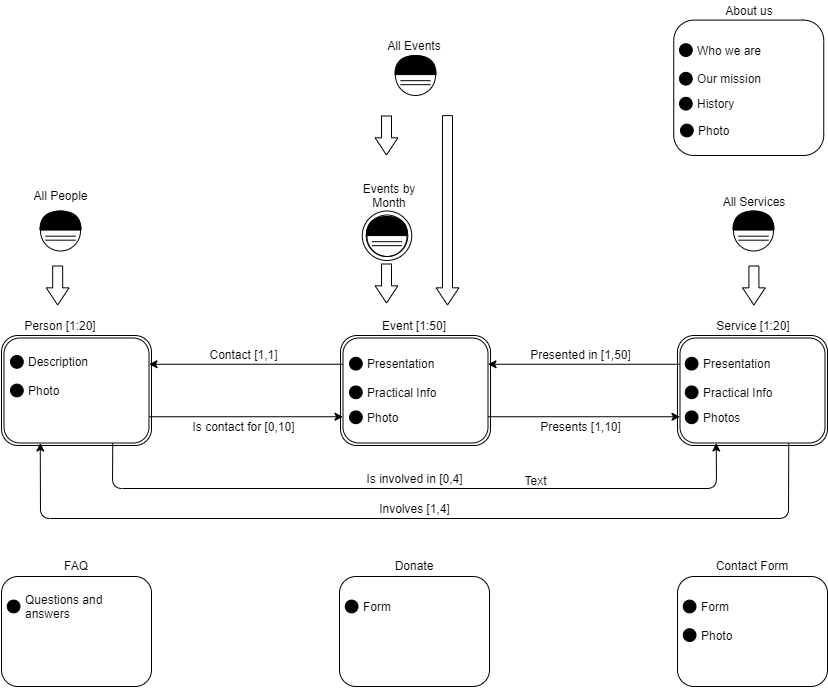
\includegraphics[width=\textwidth]{./assets/L-IDM.png}
			\caption{Logical Interactive Dialogue Model}
		\end{minipage}
	\end{figure}
	\clearpage


	%Scenarios
	\section{Scenarios}

	\subsection{Case 1}

	\subsection{Case 2}

	\subsection{Case 3}
	\clearpage


	%Design in-the-small
	\section{Design in-the-small}

	\subsection{Comments}

	\subsection{Home Page}
	...
	\clearpage


	%Database Design
	\section{Database Design}	

	\subsection{Entity Relationship Diagram}

	\subsection{Logical Design}
	\clearpage

\end{document}
